%deixar chapter vazio - exatamente como está. Preencher o documento apenaas apartir de section.
\chapter*[]{}

\section{Tema}

texto aqui

\subsection{Delimitação do tema}

texto aqui

\section{Problema}

texto aqui


\section{Objetivos}
\subsection{Objetivo Geral}
texto aqui

\subsection{Objetivos Específicos}
\begin{enumerate}
\item texto aqui
\item texto aquiã.
\end{enumerate}

\section{Justificativa}

Segundo \citeonline{bourg2013physics}, texto aqui....

\citeonline{ericson2004real} texto aqui.

texto aqui
\section{Referencial Teórico}

texto aqui

\subsection{titulo de seção}

texto aqui 

texto aqui 

\subsubsection{titulo de sub seção}
texto aqui 

texto aqui

Exemplo de Quadro com Código - veja o quadro~\ref{code:vec_1}
\begin{lstlisting}[frame=single,caption=Exemplo de vetor 3d\label{code:vec_1}]
class vector3d{
  float x;
  float y;
  float z;

  vector3d(float x, float y, float z){
    this->x=x;
    this->y=y;
    this->z=z;
  }
};
\end{lstlisting}

\subsubsection{Caixas}

uma caixa é uma caixa... veja isso na Figura~\ref{fig:figura1}

\begin{figure}[htb]
  \centering
	\caption{\label{fig:figura1} Figura mostrando uma caixa}
	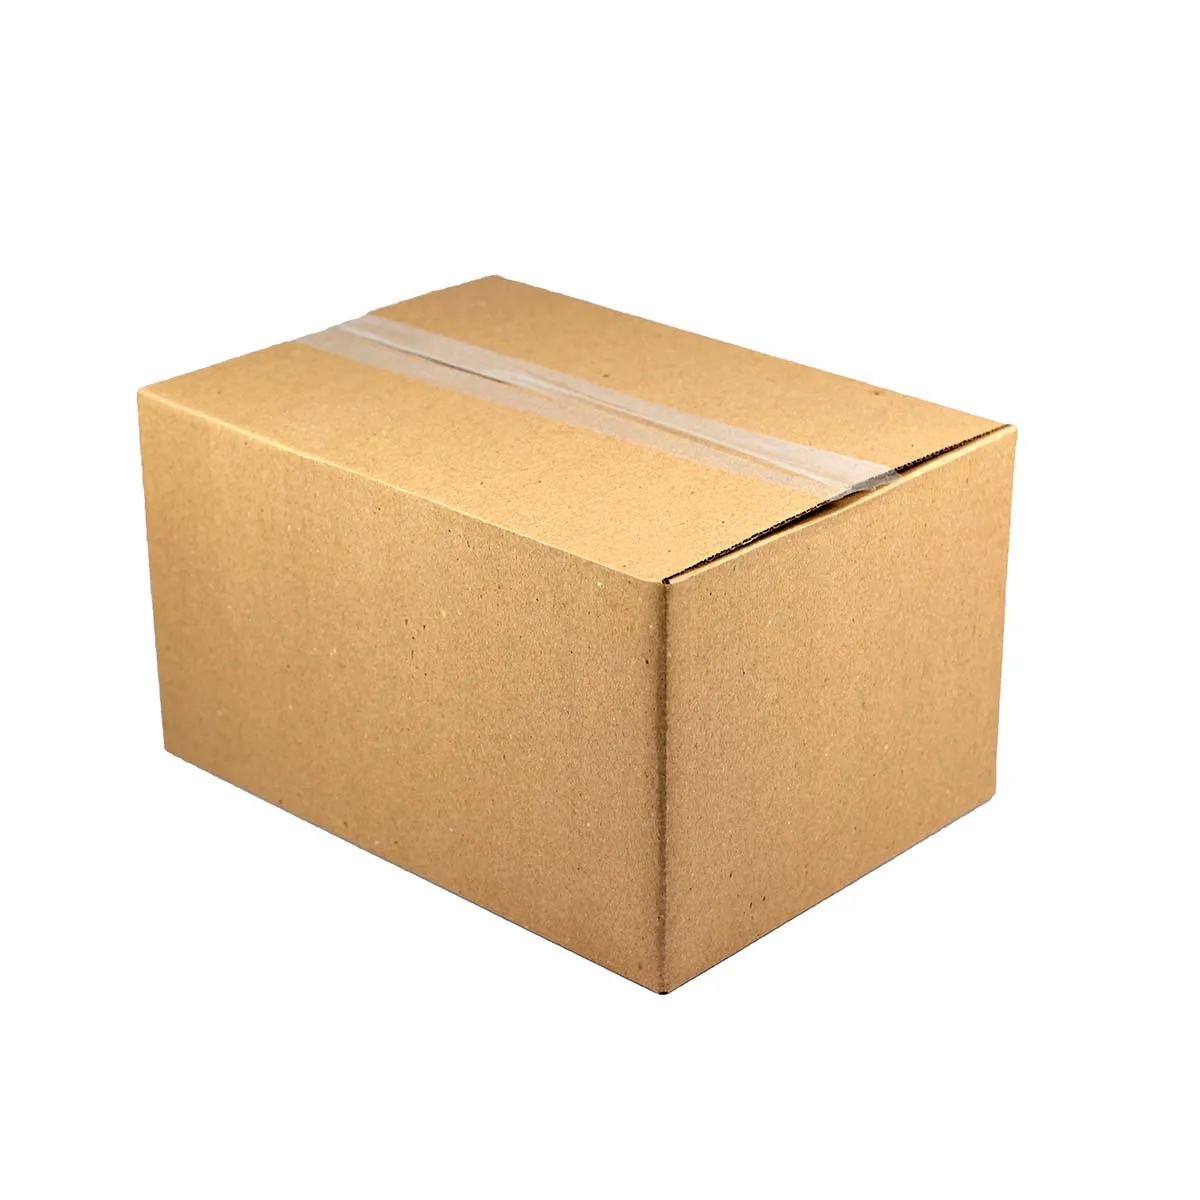
\includegraphics[scale=0.2]{Imagens/figura1.png} %width=\textwidth
	\legend{Fonte: \cite{ericson2004real}. }
\end{figure}




\section{Metodologia}

texto aqui 

\subsection{sub seção }

texto aqui 


\subsection{Recursos necessários}

Lista dos Recursos 

\begin{itemize}
\item item 1;
\item item 2;
\end{itemize}

\subsection{Cronograma}

A listagem a seguir, apresenta uma distribuição estimada das tarefas a serem
realizadas de forma quinzenal.

aqui vai o cronograma em forma de tabela.
